\documentclass[12pt]{article}

\usepackage{amsmath}
\usepackage{amsfonts}
\usepackage{tikz}
\usepackage{schemabloc}
\usetikzlibrary{calc,
                positioning,
                arrows}
\usepackage{multirow}
\usepackage{mathtools}
\usepackage{MnSymbol}
\DeclareMathOperator{\Tr}{Tr}
\usetikzlibrary{arrows}
\usepackage{chngcntr}
\counterwithin{figure}{section}
\usepackage{caption}
\usepackage{changepage}
\usepackage{subcaption}
\usepackage{xcolor}
\usepackage{listings}
\usepackage{caption}
\usepackage[normalem]{ulem}
\useunder{\uline}{\ul}{}
\usepackage{listings}           

\usepackage{answers}
\usepackage{setspace}
\usepackage{graphicx}
\usepackage{enumitem}
\usepackage{multicol}
\usepackage{mathrsfs}
\usepackage[margin=1in]{geometry} 

\begin{document}

% --------------------------------------------------------------
%                         Start here
% --------------------------------------------------------------
 
\title{Problem Set 5}%replace with the appropriate homework number
\author{Magson Gao (magson@mit.edu)\\ %replace with your name
6.111 Fall 2018} %if necessary, replace with your course title
 
\maketitle

\section{Problem A}
\begin{figure}[htb]
\centering
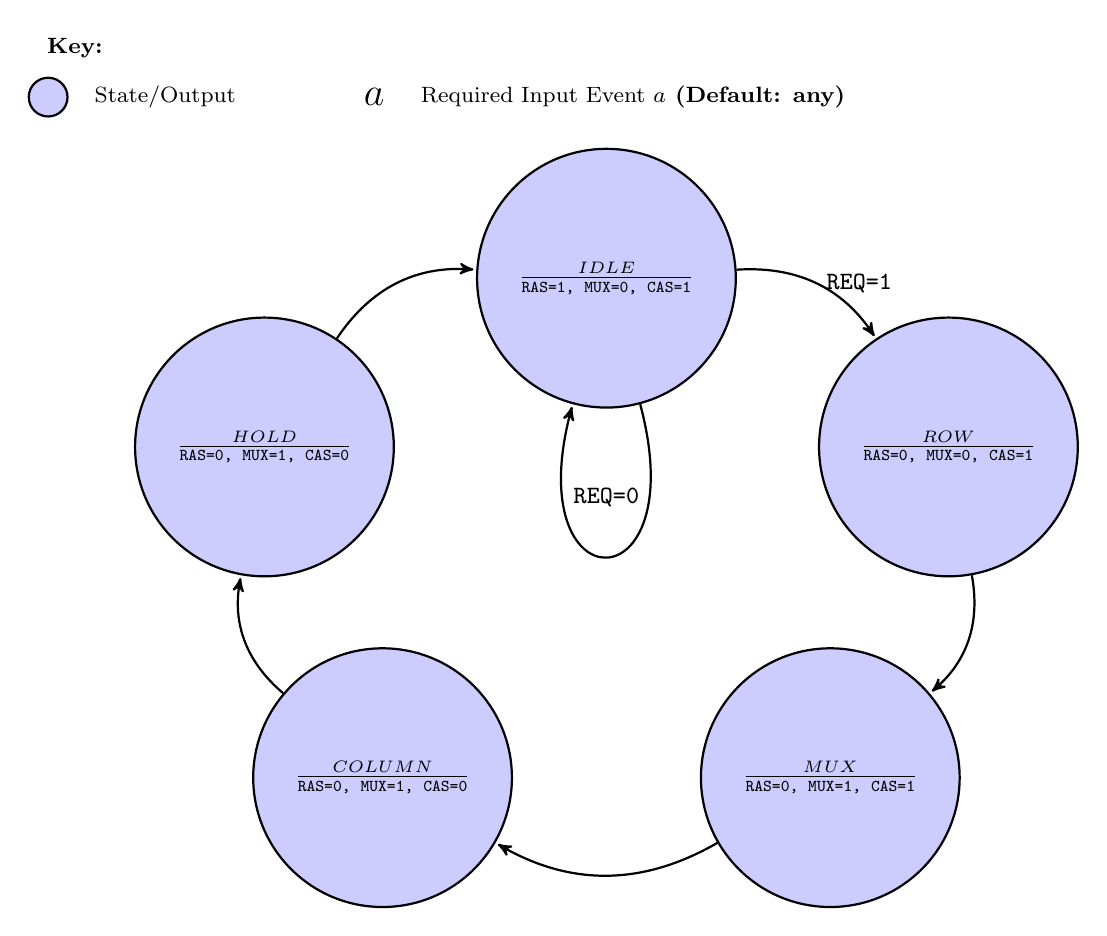
\begin{tikzpicture}[->,>=stealth',shorten >=1pt,auto,
  thick,
  key node/.style={draw=white!80,font=\footnotesize, text width=3cm, align=left},
  text node/.style={draw=white!80,font=\footnotesize, align=left},
  row node/.style={draw=white!80,font=\footnotesize,  align=left},
  main node/.style={circle,fill=blue!20,draw, font=\small\bfseries, text width=3cm, align=center}]
  \node[main node] (IDLE)  {$\frac{IDLE}{\texttt{RAS=1, MUX=0, CAS=1} }$ };
  \node[key node] (caption) [above left= 1.5cm and 2.8cm of IDLE] {\textbf{Key:}};
  \node[text node] (caption2) [below = 1mm of caption.south] {State/Output};
  \node[main node][text width=0.2cm] (caption1)  [left = 2mm of caption2]{};
  \node[text node] (caption3) [right = 12mm of caption2] {\Large$\boldsymbol{\curvearrowright}$ $a$};
  \node[text node] (caption4) [right= 2mm of caption3] {Required Input Event $a\textbf{ (Default: any)}$};
  \node[main node] (ROW) [below right =-0.2cm and 2cm of IDLE]{$\frac{ROW}{\texttt{RAS=0, MUX=0, CAS=1}}$};
  \node[main node] (MUX) [below right =4cm and 0.5cm of IDLE]{$\frac{MUX}{\texttt{RAS=0, MUX=1, CAS=1}}$};
  \node[main node] (COLUMN)  [below left =4cm and 0.5cm of IDLE]{$\frac{COLUMN}{\texttt{RAS=0, MUX=1, CAS=0} }$};
  \node[main node] (HOLD)  [below left =-0.2cm and 2cm of IDLE]{$\frac{HOLD}{\texttt{RAS=0, MUX=1, CAS=0} }$};
  \path[every node/.style={font=\small}]
      (IDLE) edge [loop below] node[below=-1cm] {$\texttt{REQ=0}$} (IDLE)
      (IDLE) edge [bend left] node[right=0cm] {$\texttt{REQ=1}$} (ROW)
      (ROW) edge [bend left] node[right=-0.5cm] {} (MUX)
      (MUX) edge [bend left] node[left=-0.5cm] {} (COLUMN)
      (COLUMN) edge [bend left] node[below left=-0.1cm and -0.5cm] {} (HOLD)
      (HOLD) edge [bend left] node[below left=-0.1cm and -0.5cm] {} (IDLE)
    ;
\end{tikzpicture}
\caption{The finite state machine diagram for the given system.}\label{fsmbuffering}
\end{figure}

\section{Problem B}
Code:
\begin{lstlisting}[
    basicstyle=\tiny,
]
module mem_controller(
            input        clk_in,
            input        req_in,
            output       ras_out,
            output       mux_out,
            output       cas_out
          );

  localparam STATE_IDLE = 3'b000;
  localparam STATE_ROW  = 3'b001;
  localparam STATE_MUX  = 3'b011;
  localparam STATE_COL  = 3'b010;
  localparam STATE_HOLD = 3'b110;

  reg [2:0] state = STATE_IDLE;

  assign ras_out = (state == STATE_IDLE);
  assign mux_out = ~((state == STATE_IDLE) | (state == STATE_ROW));
  assign cas_out = ((state == STATE_IDLE) | (state == STATE_ROW) | (state == STATE_MUX));

  // state machine
  always @(posedge clk_in)
  begin
    case (state)
      STATE_IDLE : state <= req_in ? STATE_ROW : STATE_IDLE;
      STATE_ROW  : state <= STATE_MUX;
      STATE_MUX  : state <= STATE_COL;
      STATE_COL  : state <= STATE_HOLD;
      STATE_HOLD : state <= STATE_IDLE;
    endcase
  end

endmodule
\end{lstlisting}

Testbench:
\begin{lstlisting}[
    basicstyle=\tiny,
]
`define assert(signal, value) \
        if (signal !== value) \
        begin \
            $display("ASSERTION FAILED in %m at time %0t: signal != value", $time); \
        end

module mem_controller_tb;
  reg        clk;
  reg        req;
  wire       ras;
  wire       mux;
  wire       cas;
  reg [2:0]  clk_counter;

  initial
  begin
      $dumpfile("test.vcd");
    $dumpvars(0,mem_controller_tb);
    clk         = 0;
    clk_counter = 0;
    req         = 0;
    
    #2;
    req = 1;
    
    #11;
    req = 0;
    #50;
    $finish;
  end


  mem_controller m1(
            .clk_in    (clk),
            .req_in    (req),
            .ras_out   (ras),
            .mux_out   (mux),
            .cas_out   (cas)
            );

  always @(posedge clk)
  begin
    if ((clk_counter > 0) | ((req == 1) & (clk_counter == 0)))
    begin
      clk_counter = clk_counter + 1;

      if (clk_counter == 1)
      begin
        `assert(ras, 0);
        `assert(mux, 0);
        `assert(cas, 1);        
      end
      else if (clk_counter == 2)
      begin
        `assert(ras, 0);
        `assert(mux, 1);
        `assert(cas, 1);        
      end
      else if (clk_counter == 3)
      begin
        `assert(ras, 0);
        `assert(mux, 1);
        `assert(cas, 0);
      end
      else
      begin
        `assert(ras, 0);
        `assert(mux, 1);
        `assert(cas, 0);
        clk_counter = 0;
      end
    end
  end

  always #5 clk = ~clk;

endmodule
\end{lstlisting}

\section{Problem C}
It is glitch free as the states are encoded using grey codes, thus all change of states except from state hold to state idle requires only one bit change. For state hold to state idle there are two possible glitches: 110 to 100 to 000 or 110 to 010 to 000. In both cases the intermediate meta-state has identical output values to the initial hold state. Thus no output glitches occur.
\section{Problem D}
\begin{figure}[!b]
  \centering
  \includegraphics[width=0.9\linewidth]{screen.png}
\end{figure}

\end{document}
